\documentclass{article}
\usepackage{pifont}  % 提供文件夹和文件的图标
\usepackage{xcolor}  % 设置颜色
\usepackage{tikz}
\usetikzlibrary{positioning}
\usepackage[section]{placeins}
\usetikzlibrary{positioning, arrows}

\newcommand{\folder}{\textcolor{blue}{\ding{117}}}  % 文件夹图标
\newcommand{\file}{\textcolor{black}{\ding{115}}}    % 文件图标


\begin{document}



\section{Instruction to the Framework}

\subsection{Overview of the Framework's Architecture}


This part provides an overview of the organization and layout of the files within the system. It explains how files are structured, including directory hierarchies.

\begin{itemize}
  \item Root Directory
    \begin{itemize}
      \item  SRC
        \begin{itemize}
          \item  \textbf{main1.cpp} \quad \textcolor{black}{\small example usage1}
          \item  \textbf{main2.cpp} \quad \textcolor{black}{\small example usage2}
          \item  \textbf{main3.cpp} \quad \textcolor{black}{\small example usage3}
          \item  \textbf{main4.cpp} \quad \textcolor{black}{\small example usage4}
          \item  \textbf{main5.cpp} \quad \textcolor{black}{\small example usage5}
          \item  framwork
            \begin{itemize}
              \item  \textbf{graphnode.h} \quad \textcolor{black}{\small graph node definition header file}
              \item  \textbf{graphnode.cc} \quad \textcolor{black}{\small graph node implementation}
              \item  \textbf{niobase.h} \quad \textcolor{black}{\small NIO data, a struct data that can be shared between different graph nodes}
              \item  \textbf{register.h} \quad \textcolor{black}{\small register each graph node}
              \item  \textbf{register.cc} \quad \textcolor{black}{\small register each graph node(implementation)}
              \item  \textbf{registerdata.h} \quad \textcolor{black}{\small register NIO data, header file}
              \item  \textbf{registerdata.cc} \quad \textcolor{black}{\small register NIO data, implementation}
              \item  \textbf{util.h} \quad \textcolor{black}{\small some utility function, header file}
              \item  \textbf{util.cc} \quad \textcolor{black}{\small some utility function, implementation}
            \end{itemize}
        \end{itemize}

      \item DATA
        \begin{itemize}
          \item \textbf{a.out} \quad \textcolor{black}{\small exe to generate input data}
          \item \textbf{data.csv} \quad \textcolor{black}{\small input data}
          \item \textbf{main.cpp} \quad \textcolor{black}{\small source code to generate input}
          \item \textbf{output1\_from\_EXE4.csv} \quad \textcolor{black}{\small output1 from EXE4}
          \item \textbf{output\_from\_EXE4.csv} \quad \textcolor{black}{\small output from EXE4}
          \item \textbf{output\_from\_EXE5.csv} \quad \textcolor{black}{\small output from EXE5}
          \item \textbf{output\_from\_EXE2.csv} \quad \textcolor{black}{\small output from EXE2}
          \item \textbf{output\_from\_EXE3\_AAPL.csv} \quad \textcolor{black}{\small output from EXE3\_AAPL}
          \item \textbf{output\_from\_EXE3\_GOOG.csv} \quad \textcolor{black}{\small output from EXE3\_GOOG}
          \item \textbf{output\_from\_EXE3\_JPM.csv} \quad \textcolor{black}{\small output from EXE3\_JPM}
        \end{itemize}
      \item \textbf{CMakeLists.txt} \quad \textcolor{black}{\small CMake configuration file}
      \item \textbf{README.txt} \quad \textcolor{black}{\small readme file}
    \end{itemize}
\end{itemize}


Next, let's introduce several important files and how the framework operates.


\subsubsection{graphnode.h}


GraphNodeBase is a virtual base class, and \textbf{all nodes on the computation graph inherit from this base class}. It has two important virtual functions: one is Initialize, used to initialize each node and register the data used; the other is LoadData, where users need to implement the specific computation logic.
\begin{figure}[h]
\centering
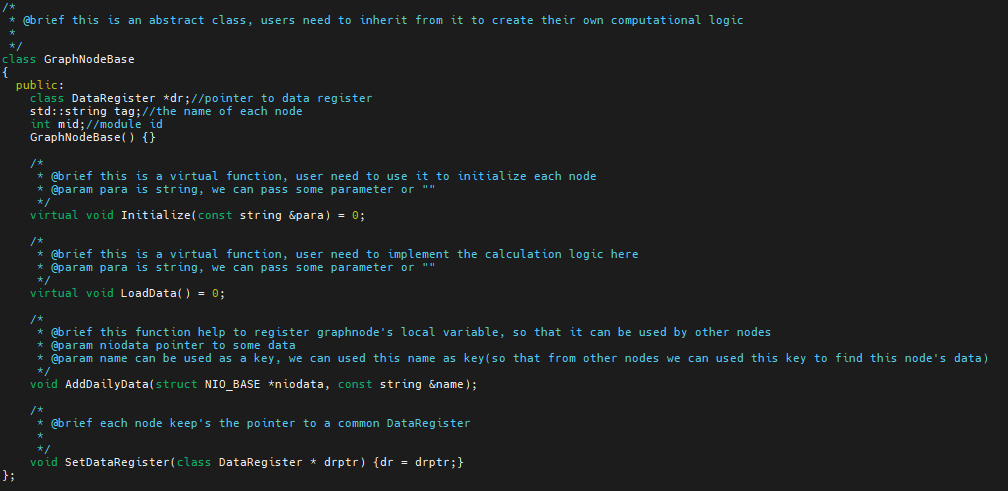
\includegraphics[height=180pt]{IMG/26.PNG}
\centering
\caption {GraphNodeBase}
\end{figure}


\FloatBarrier

\subsubsection{niobase.h}

NIO\_BASE is \textbf{an abstract class related to data}. Its purpose is to allow each node to define different types of data inherited from the NIO\_BASE class. Each graph node can access data from other nodes through a unified interface.
\begin{figure}[h]
\centering
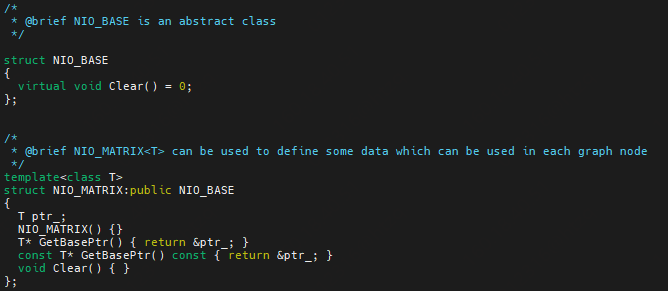
\includegraphics[height=140pt]{IMG/27.PNG}
\centering
\caption {NIO\_BASE}
\end{figure}


\FloatBarrier

\subsubsection{register.h}

The Register class is used to \textbf{manage the registration of all nodes}. The register.h file provides a REGISTER macro, which facilitates the generation of specific node objects using class name strings. For example, if we implement a graph node class name GraphNode1, GetClassFromName("GraphNode1") will return a pointer to an object with type GraphNode1.
\begin{figure}[h]
\centering
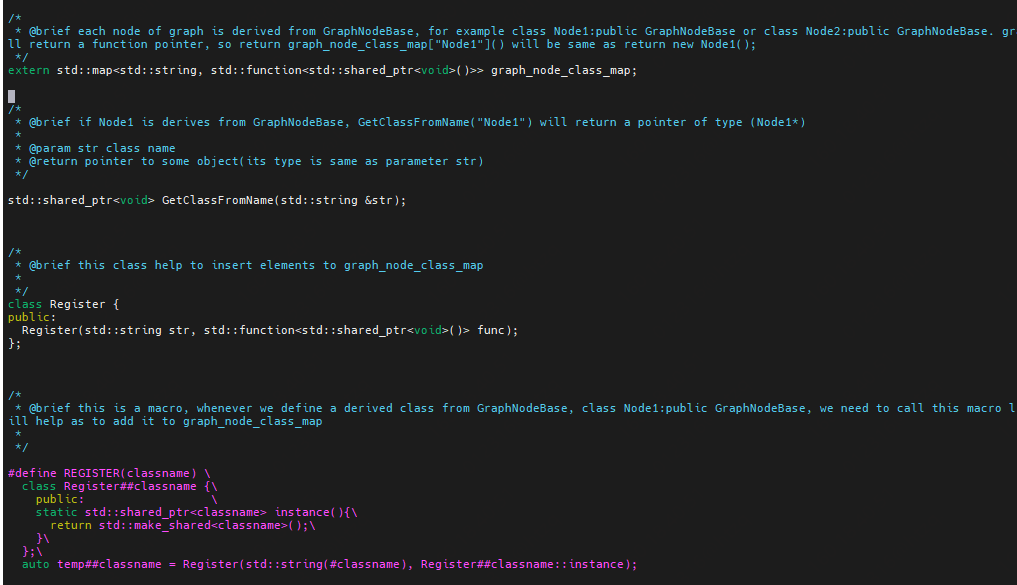
\includegraphics[height=200pt]{IMG/28.PNG}
\centering
\caption {Register}
\end{figure}

\FloatBarrier

\subsubsection{registerdata.h}

The RegisterData class is used to \textbf{manage the registration of the NIO\_DATA class}. Only registered data can be shared across different graph nodes. We can obtain the registered data through the GetData method.
\begin{figure}[h]
\centering
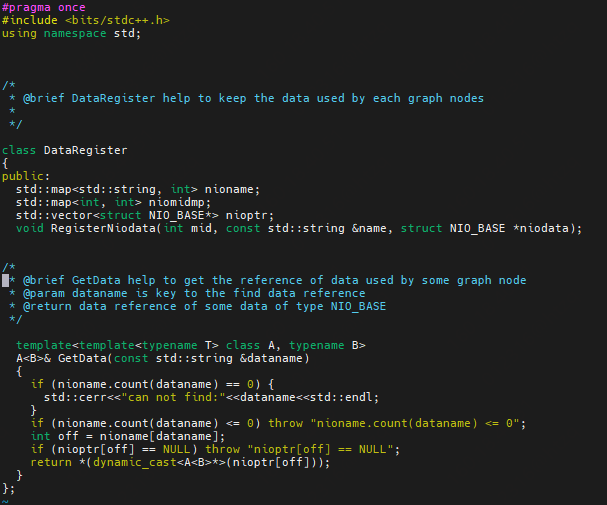
\includegraphics[height=280pt]{IMG/29.PNG}
\centering
\caption {RegisterData}
\end{figure}



\FloatBarrier

\subsubsection{How Does the Framework Work}


What the user should do:


\begin{itemize}
  \item User needs to \textbf{implement graph nodes}(inherit from GraphNodeBase defined in graphnode.h), register.h will help to create the node object.
  \item If some node has data to be shared by other nodes, we need to \textbf{store it in structure NIO\_BASE}(noibase.h), and register it with class RegisterData(registerdata.h)
  \item The computation \textbf{graph should be a DAG}, and we can use toposort to get the correct update order.
  \item When we need to update the graph, \textbf{update each node in topological order}.
\end{itemize}


What the framework do for us:

\begin{itemize}
  \item Use a vector of pointer of GraphNodeBase to manage all the user defined nodes.
  \item Use a DataRegister to manage the data that shared between graph nodes.
  \item Update each node in topological order.
\end{itemize}



\subsection{Introduction to Testing Data}

We generate the testing data by using following code.
\begin{figure}[h]
\centering
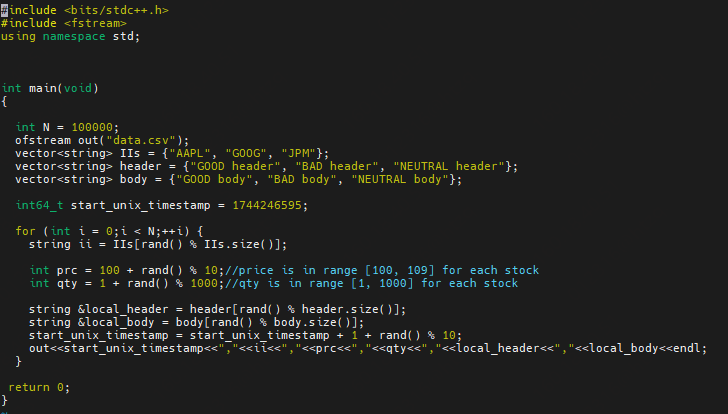
\includegraphics[height=180pt]{IMG/24.PNG}
\centering
\caption {code to generate testing data}
\end{figure}

\FloatBarrier

Followings are \textbf{some assumptions} we make about the data.

\begin{itemize}
  \item There are 6 columns in total, timestamp, ticker, price, volume, headline, body of news.
  \item To make it simple, we use the unix timestamp.
  \item There are only 3 type of headlines: "GOOD header", "BAD header", "NEUTRAL header".
  \item There are only 3 type of body of news: "GOOD body", "BAD body", "NEUTRAL body".
  \item There are only 3 type of instruments: "AAPL", "GOOG", "JPM".
  \item To simplify, we randomly create a new record with random ticker.
  \item To simplify, price and volume are some random variable in certain range.
\end{itemize}


\subsection{How to Compile and Run The Code}

To install and build the project, follow these steps:

\subsubsection{Install cmake and g++}

Make sure your machine has cmake and g++


\subsubsection{Navigate to the project directory}
cd [project-name]


\subsubsection{Create a build directory}
mkdir build; cd build\\\\
if build exists, suggest remove it first.


\subsubsection{Run CMake to configure the project}
cmake ..


\subsubsection{Build the project}
make
(or make -j20)


If everything is correct, we can successfully compile the project.
\FloatBarrier
\begin{figure}[h]
\centering
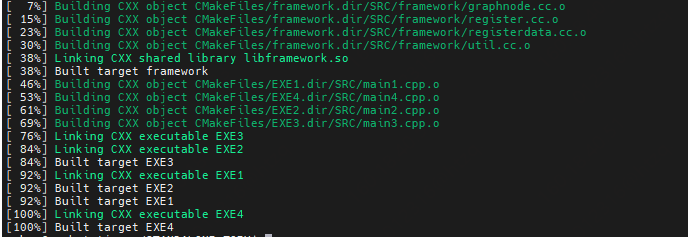
\includegraphics[height=120pt]{IMG/25.PNG}
\centering
\caption {output of compiling}
\end{figure}


\subsubsection{Run different examples}
After building the project, you can run the executable from the build directory:\\

there are 5 different examples:\\

\begin{itemize}
  \item ./build/EXE1 (define some graph nodes, calculating some PV features when good news or bad news happens, only for AAPL)\\
  \item ./build/EXE2 (define some graph nodes, calculating some PV features when good news or bad news happens, and save features for AAPL)\\
  \item ./build/EXE3 (define some graph nodes, calculating some PV features when good news or bad news happens, and save features for more than one instruments)\\
  \item ./build/EXE4 (this example is a more complex version, adding a graph node showing how to calculate a groupby algo in a stream way, and adding a node keep the feature when an hourly event happens)\\
  \item ./build/EXE5 (not related to event processing, showing other usage)\\

\end{itemize}


In next section, will explain each of these four examples.



%%%%%%%%%%%%%%%%%%%%%%%%%%%%%%%%%%%%%%%%%%%%%%%%%%%%%%%%%%%%%%%%

\newpage
\section{Examples Showing How to Use the Framework}

Here, five examples are provided, each located in main1, main2, main3, and main4, main5, respectively. These examples demonstrate different usage scenarios or approaches of the framework. They are independent code segments with some connections between them.



\begin{itemize}
  \item main1: Illustrates how to add computation nodes, establish topological relationships, and perform calculations.
  \item main2: Builds upon main1 by introducing a new node that saves features.
  \item main3: Shows how to handle multiple stocks simultaneously.
  \item main4: Further extends main2 by adding more computation nodes and demonstrating the implementation of groupby logic in a streaming context.
  \item main5: Shows how to apply operations on some dataframe, which is useful for data mining.
\end{itemize}


Each example focuses on a specific aspect of the framework, providing a comprehensive understanding of its capabilities and flexibility.



\subsection{main1.cpp}


This section demonstrates how to \textbf{define the nodes of a graph, establish dependencies between nodes, generate the execution order of the nodes, and calculate all nodes in order} when there is information update. In this example, we assume that we are only processing the stock AAPL.




\FloatBarrier
\subsubsection{step 1 define graph node}

Each graph node's calculation logic is different, so for each node we need to implement its logic. Following are some rules we need to obey.


\begin{itemize}
  \item we can use NIO\_DATA to define member variables, then it can be visited by other nodes
  \item if we define some NIO\_DATA, we need to initialize it in Initialize function
  \item if we need to visit data from other graph nodes, we can use function GetData
  \item need to design the calculation carefully
  \item need to call the REGISTER at the end of definition
\end{itemize}


Here is an example of calculating the average price. Each time a new price data point is observed, we need to maintain the cumulative sum and the count of all samples observed so far. The average price is then obtained by dividing the cumulative sum by the count.

\begin{figure}[h]
\centering
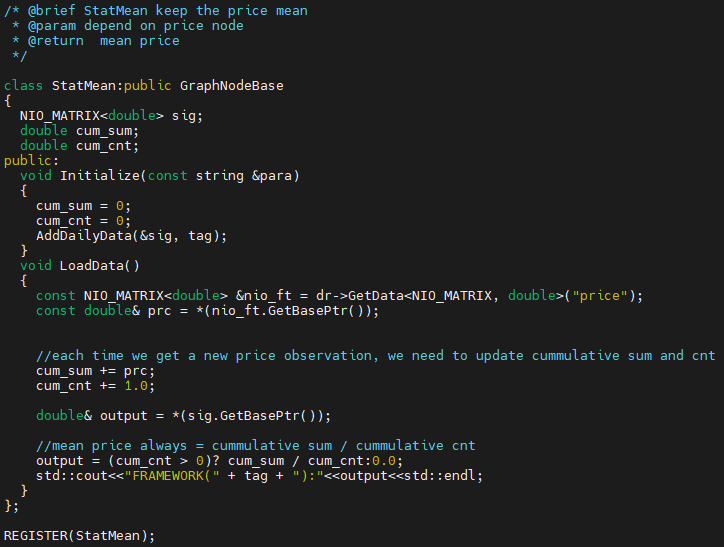
\includegraphics[height=250pt]{IMG/0.PNG}
\centering
\caption {example of mean price}
\end{figure}




\FloatBarrier
\subsubsection{step 2 store node names and class names}

We assume that we have completed the code for all the classes of the graph nodes. We need to record them using arrays, where their names (which can be arbitrarily assigned) and the specific class names are recorded in two separate arrays.

\begin{figure}[h]
\centering
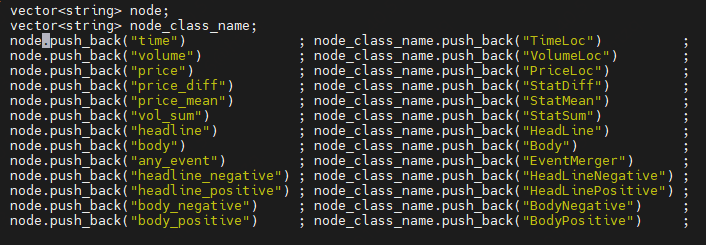
\includegraphics[height=120pt]{IMG/1.PNG}
\centering
\caption {store node names}
\end{figure}




\FloatBarrier
\subsubsection{step 3 add dependencies}
Next, we add dependencies between the nodes based on the required computation order. Each node may depend on several other nodes or may have no dependencies at all. It is important to note that this directed graph should not have any cycles; otherwise, the computation cannot be completed.

\begin{figure}[h]
\centering
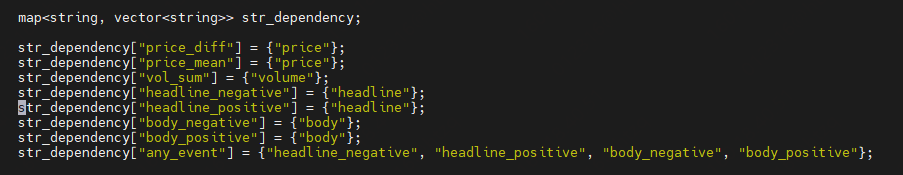
\includegraphics[height=70pt]{IMG/2.PNG}
\centering
\caption {add dependencies}
\end{figure}


\FloatBarrier
Here is the structure of the generated graph. The 'time' node has no dependencies, while the 'any\_event' node depends on four other nodes.

\begin{figure}[h]
\centering
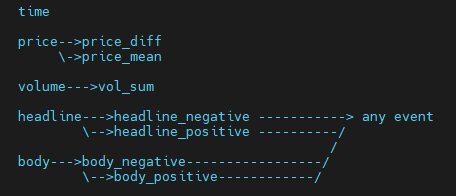
\includegraphics[height=120pt]{IMG/3.PNG}
\centering
\caption {structure of the generated graph}
\end{figure}

\FloatBarrier
\subsubsection{step 4 create object for each graph node}

Then, we need to create objects for each node in the graph. Additionally, we need a DataRegister class to manage the data that can be shared among the graph nodes.

\begin{itemize}
  \item due to C++ polymorphism, we can use an array of GraphBase base class pointers to record all node objects.
  \item eche node has a unique name.
  \item each node keeps the pointer to DataRegister
\end{itemize}



\begin{figure}[h]
\centering
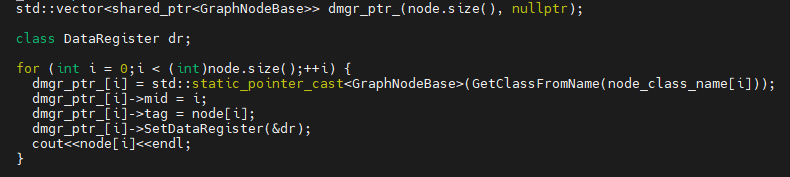
\includegraphics[height=80pt]{IMG/4.PNG}
\centering
\caption {create object for each graph node}
\end{figure}


\FloatBarrier
\subsubsection{step 5 call Initialize function for each node}
For each node, calling the Initialize function once completes data registration and sets up the initial state.
\begin{figure}[h]
\centering
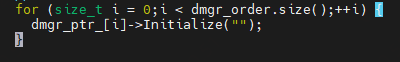
\includegraphics[height=40pt]{IMG/5.PNG}
\centering
\caption {call Initialize function for each node}
\end{figure}


\FloatBarrier
\subsubsection{step 6 update the graph}

For each piece of related data, the LoadData function is called according to the node invocation order. In this example, we focus solely on the calculation of features for a single stock and the definition of events. Subsequent examples will involve more complex scenarios.

\begin{figure}[h]
\centering
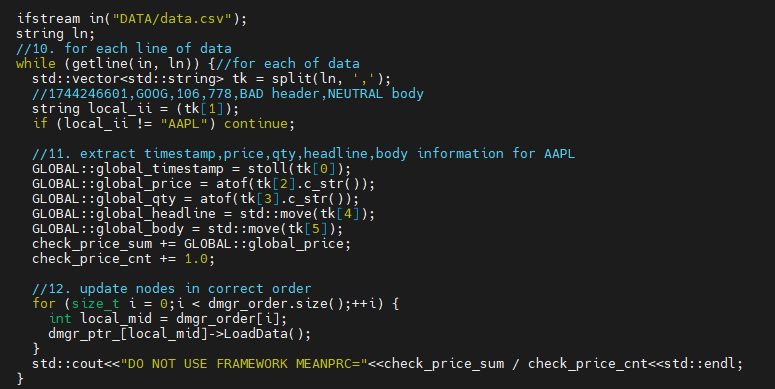
\includegraphics[height=180pt]{IMG/7.PNG}
\centering
\caption {update the graph when we recieve a new record}
\end{figure}



\FloatBarrier
\subsection{main2.cpp}

The second example demonstrates how to extend the first example. For instance, if you want to \textbf{record the current time and some features when an event occurs and save the information into a specific file}, you can follow these steps to achieve it.


\FloatBarrier
\subsubsection{design a new graph node class}


Based on main1, the goal of main2 can be achieved by making some extensions.\\

First, design a new class, FeatureDumper, to record specific information (such as timestamp, price\_diff, price\_mean, and vol\_sum) when the event flag is set to 1.

\begin{figure}[h]
\centering
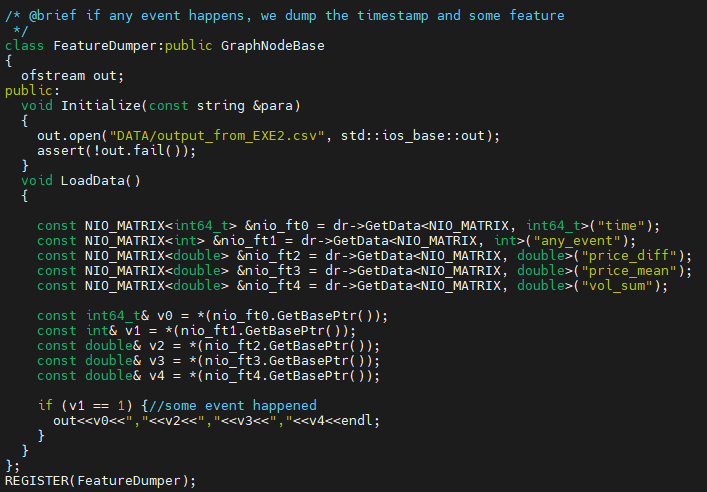
\includegraphics[height=250pt]{IMG/10.PNG}
\centering
\caption {design a new class}
\end{figure}


\FloatBarrier
\subsubsection{add node information to graph}

Add a node to the graph with name feature\_dumper.


\begin{figure}[h]
\centering
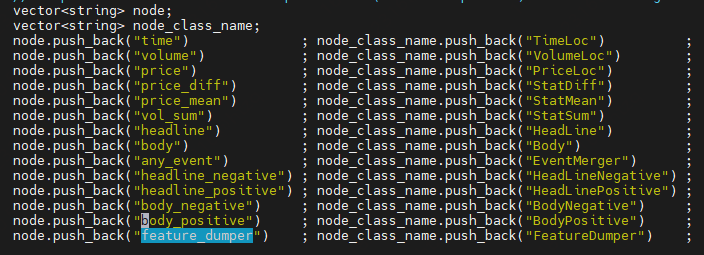
\includegraphics[height=80pt]{IMG/8.PNG}
\centering
\caption {add new node to graph}
\end{figure}

\FloatBarrier
\subsubsection{add new dependency}


Add dependency relationships, as the new node depends on the time, price\_diff, price\_mean, vol\_sum, and any\_event nodes, requiring these dependencies to be incorporated.


\begin{figure}[h]
\centering
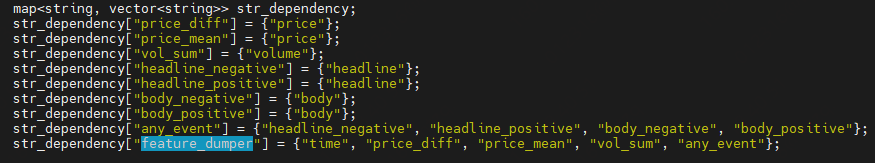
\includegraphics[height=80pt]{IMG/9.PNG}
\centering
\caption {add new dependency}
\end{figure}

\FloatBarrier



The structure of the graph becomes more complex after the update.


\begin{figure}[h]
\centering
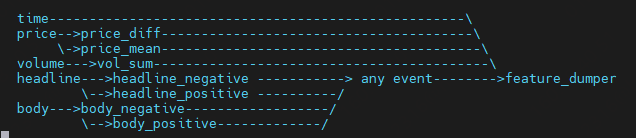
\includegraphics[height=80pt]{IMG/11.PNG}
\centering
\caption {graph is more complex}
\end{figure}


\FloatBarrier
\subsubsection{update the graph and check the result}


Run the program again, and it will record the current timestamp and volume-price features at the event occurrence, writing them into the file DATA/output\_from\_EXE2.csv. It has 4 columns in total, timestamp, price diff, mean price and cumulative volume. It only records the timestamp when any positive or negative event happens(skip neutral one).
\begin{figure}[h]
\centering
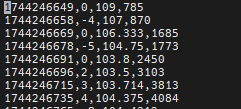
\includegraphics[height=100pt]{IMG/30.PNG}
\centering
\caption {run the program again and will get the output file}
\end{figure}



\FloatBarrier
\subsection{main3.cpp}

The previous two examples handled the situation for a single stock. This example demonstrates how to \textbf{handle multiple stocks}. Since each stock is independent, we can add a computation graph for each stock, but to achieve this, some adjustments need to be made.




\FloatBarrier
\subsubsection{change some graph node class}


For some input and ouput graph node, we need to keep the information of stock id, this stock id information can be used to the graph node to get the corret input and make the correct output. We need to modify the Initialize function a little bit.(following is the vimdiff between old and new)

\begin{figure}[h]
\centering
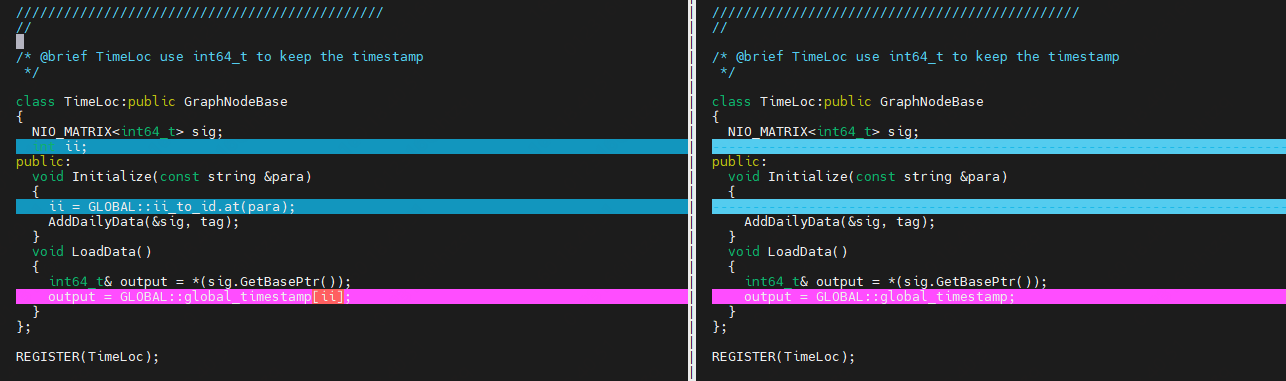
\includegraphics[height=100pt]{IMG/13.PNG}
\centering
\caption {change some the graph node class code}
\end{figure}

\FloatBarrier

\begin{figure}[h]
\centering
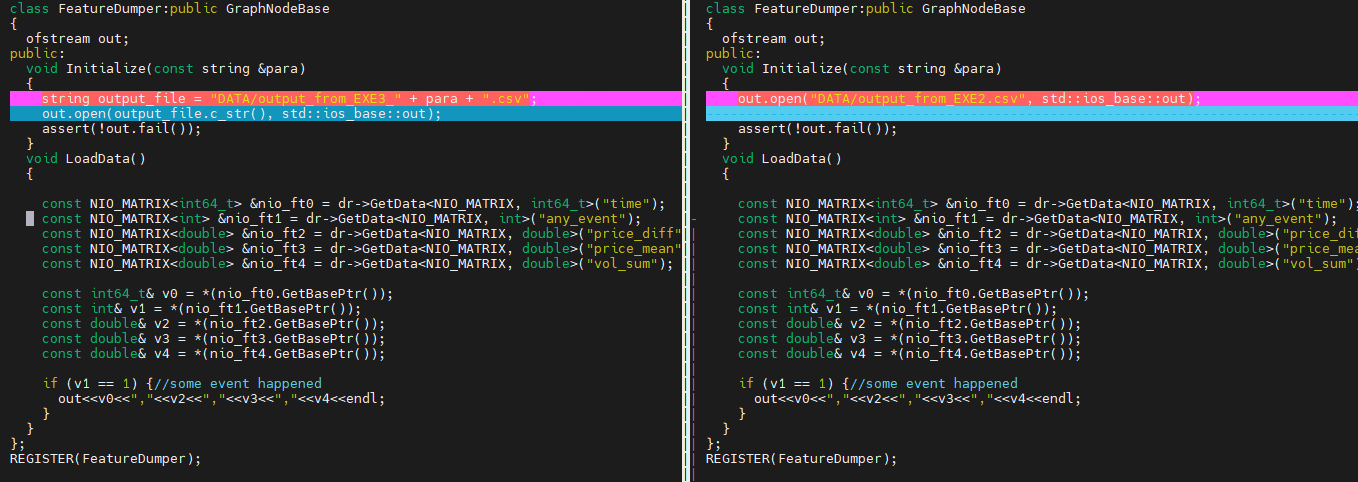
\includegraphics[height=120pt]{IMG/14.PNG}
\centering
\caption {for the dumper we add ticker information to output file name}
\end{figure}

\FloatBarrier



\FloatBarrier
\subsubsection{for each stock create a graph}

Although we do not need to modify the topology of the graph, we need to \textbf{add the entire graph structure and an independent DataRegister} for each stock.


\begin{figure}[h]
\centering
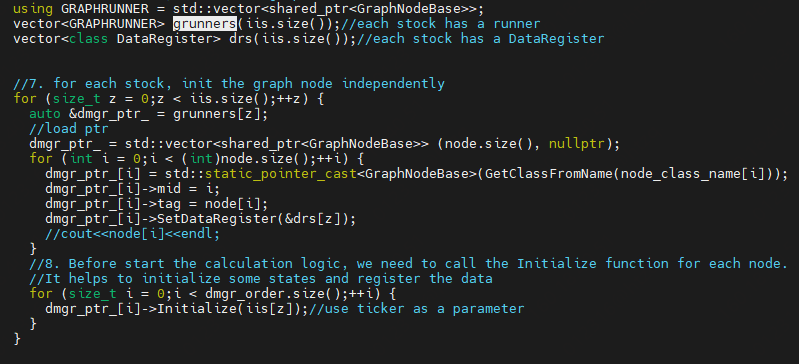
\includegraphics[height=180pt]{IMG/15.PNG}
\centering
\caption {for each stock create a graph}
\end{figure}

\FloatBarrier
\subsubsection{each stock one graph}


For each new record, \textbf{find the corresponding graph for the current stock} and update the information.


\begin{figure}[h]
\centering
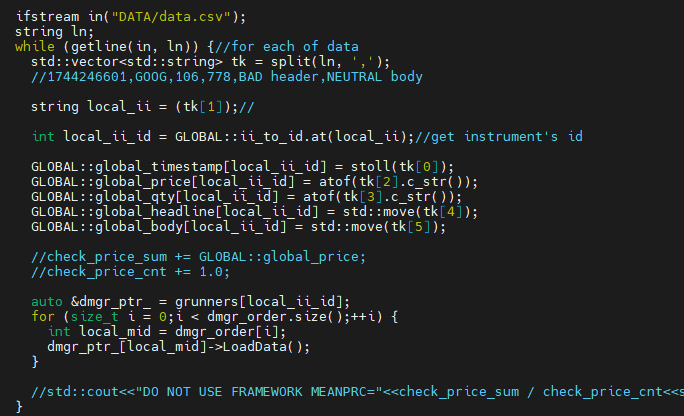
\includegraphics[height=150pt]{IMG/16.PNG}
\centering
\caption {update the graph}
\end{figure}

\FloatBarrier



Three different files will be generated to record the volume-price features and event timestamps for each stock when an event occurs.


\begin{figure}[h]
\centering
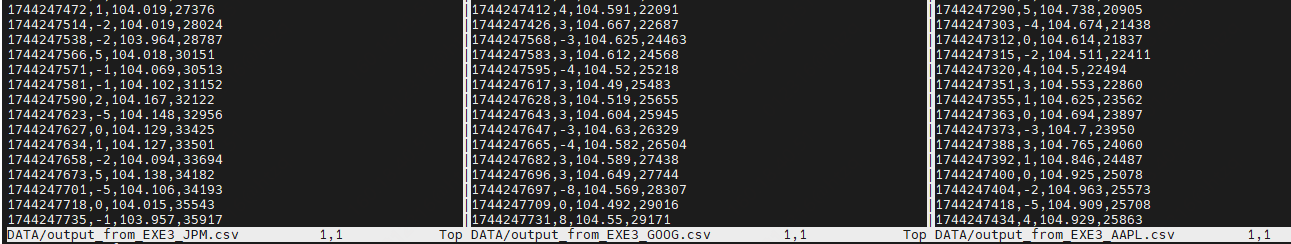
\includegraphics[height=70pt]{IMG/17.PNG}
\centering
\caption {output for each stock}
\end{figure}


%%%%%%%%%%%%%%%%%%%%%%%%%%%%%%%%%%%%%%%%%%%%%

\FloatBarrier
\subsection{main4.cpp}


In practice, we may need more complex computational logic and record samples corresponding to different events. This example demonstrates how to add a \textbf{groupby-related operator} and how to \textbf{simultaneously record multiple events} if needed.




\FloatBarrier
\subsubsection{a groupby\_mean\_std operator}


As before, we need to add a groupby\_mean\_std-related operator(df[['price', 'volume']].groupby(by='price').mean().std()). In a streaming computation scenario, we need to record some states, such as \textbf{the sum and count of occurrences for each key}, as well as the \textbf{total count, total sum, and sum of squares for all keys}. For each new data point, we can update the relevant numerical values. 


\begin{itemize}
  \item For each key(price), we need to maintain its mean volume.
  \item We can use gbsum\_cnt to keep each key(price)'s cumulative volume and count. So we can find the mean by deviding them.
  \item In order to find the std of all key's mean volume, we need to keep its mean(variable 'up' in the code), squre mean (variable 'up2' in the code)and count.
  \item for any new record, there will be two possible cases.
  \item (1) if the record's price \textbf{is not in gbsum\_cnt}, we add (qty, 1) to gbsum\_cnt, this new key's mean is v = gbsum\_cnt / 1, so update up=up+v, up2 = up2 + v * v;
  \item (2) if the record's price \textbf{is alreadly in gbsum\_cnt}, we adjust gbsum\_cnt[current price] by (qty, 1) , and change up and up2 in a different way, For details, see the code.

  \item Finally, the std can be found by using the information of the latest up, up2 and the size of gbsum\_cnt.
  
  

\end{itemize}


\begin{figure}[h]
\centering
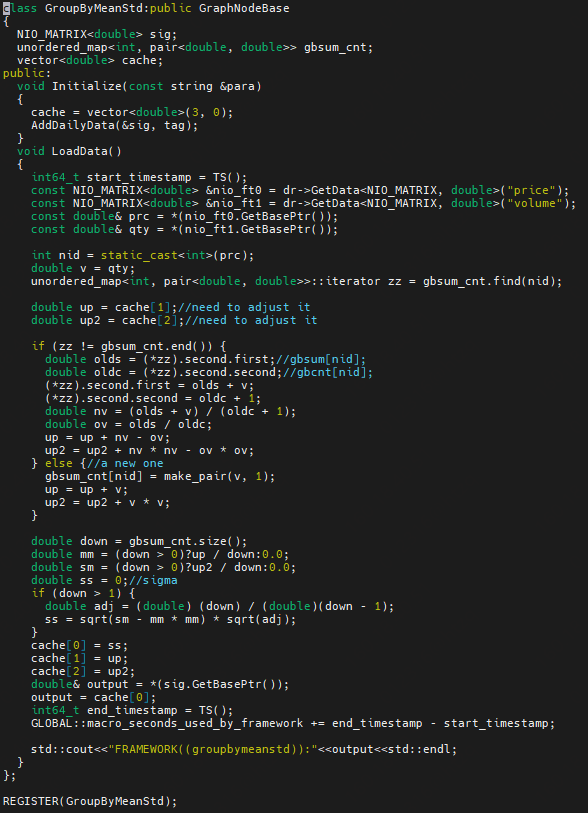
\includegraphics[height=370pt]{IMG/18.PNG}
\centering
\caption {a groupby\_mean\_std operator}
\end{figure}

\FloatBarrier


We also need a node which reads in time stamp and detect the transition to a new hour. (This is an hourly event, 1 if the timestamp first time gets into a new hour, other case 0)


\begin{figure}[h]
\centering
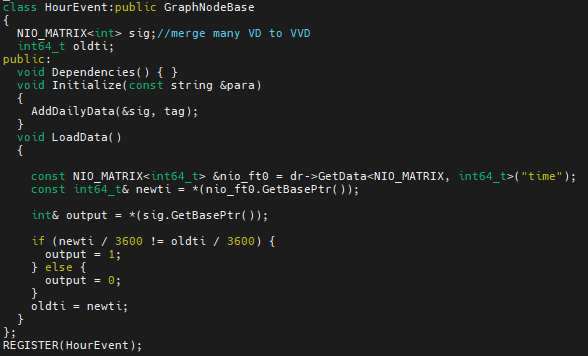
\includegraphics[height=200pt]{IMG/19.PNG}
\centering
\caption {for the dumper we add ticker information to output file name}
\end{figure}

\FloatBarrier



\FloatBarrier
\subsubsection{structure of the graph}


The final generated topology is more complex than before, and in this example, we also write groupby-related factors as features into the file.


\begin{figure}[h]
\centering
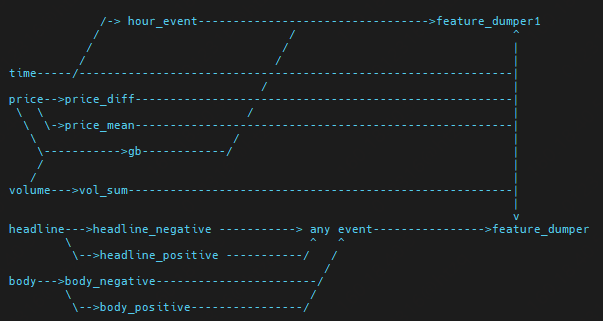
\includegraphics[height=140pt]{IMG/20.PNG}
\centering
\caption {structure of the graph}
\end{figure}

In summary, there are \textbf{two types of events} in the graph:
\begin{itemize}
  \item any\_event(any news related event), if any positive news or negative news or positive body or negative body event happens, we set any\_event to 1.
  \item hour\_event, if enter an new hour, we set it to 1.
\end{itemize}

There are \textbf{four price volume related features}:

\begin{itemize}
  \item price\_diff:price diff
  \item price\_mean:price mean
  \item vol\_sum:sum of volume
  \item gb : df[['price', 'volume']].groupby(by='price').mean().std()
\end{itemize}

There are \textbf{two feature dumpers}:
\begin{itemize}
  \item feature\_dumper1:dump hour\_event related feature
  \item feature\_dumper:dump new event related feature
\end{itemize}



\FloatBarrier
\subsubsection{update the graph}


At each update, we can directly compute to verify whether the framework provides the correct results.
For each event, the code print two lines to the sceen, one is the feature score by using the framework, another one
is the feature score we calculate without the framework. \textbf{If everything is correct, those two scores should be
the same}.


\begin{figure}[h]
\centering
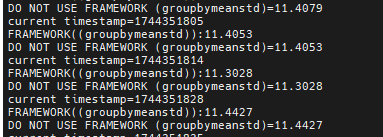
\includegraphics[height=100pt]{IMG/31.PNG}
\centering
\caption {two methods to find groupbymeanstd}
\end{figure}

\FloatBarrier


As expected, this program generates two output files. One is related to news event timestamps, and the other is related to hourly events (including groupby features, so an additional column is added).


\begin{figure}[h]
\centering
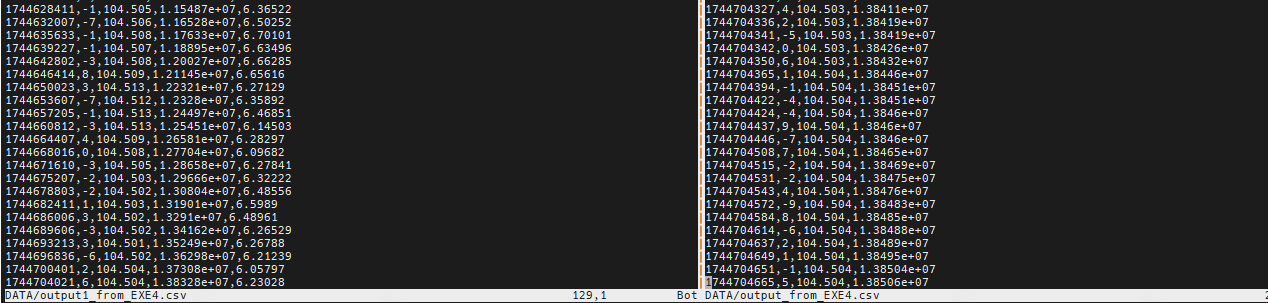
\includegraphics[height=80pt]{IMG/22.PNG}
\centering
\caption {output files}
\end{figure}


\FloatBarrier


Additionally, the program prints out the total time consumption of two calculation methods at the end, and it can be seen that the time consumption of stream processing is \textbf{significantly less} than that of direct calculation.


\FloatBarrier
\begin{figure}[h]
\centering
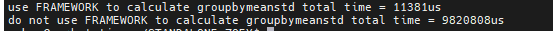
\includegraphics[height=20pt]{IMG/23.PNG}
\centering
\caption {time comparison}
\end{figure}



\FloatBarrier
\subsection{main5.cpp}


This part provides an example that is not closely related to event-driven architecture. In this example, we demonstrate \textbf{how to handle operations related to DataFrames} using this framework. We want to do following things: \textbf{based on one dataframe as input, try to extract four differnt features from it and save in csv}.Here, we present a new operator example based on DataFrames.(for details, please refer to source code)


\begin{figure}[h]
\centering
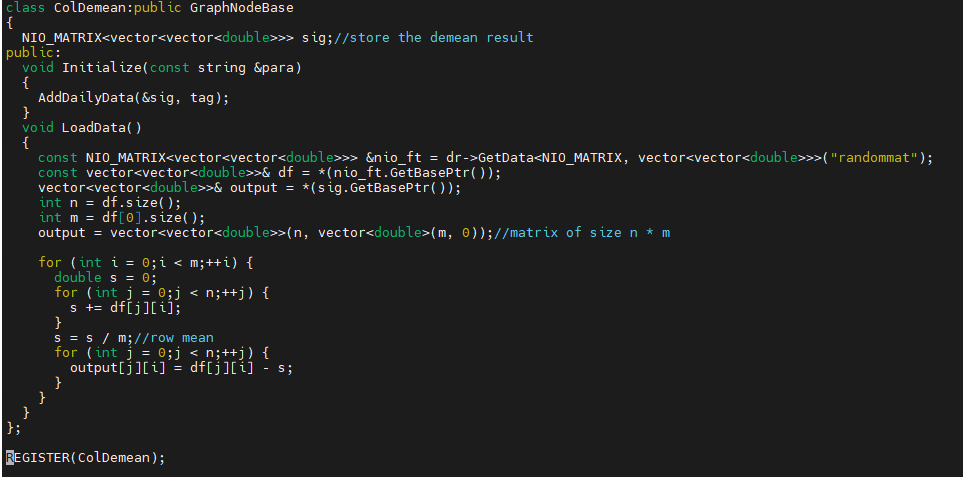
\includegraphics[height=180pt]{IMG/35.PNG}
\centering
\caption {new node related to dataframe op}
\end{figure}

\FloatBarrier



We create a different computation graph in this example. Based on one random matrix as input, we apply some opertions on it(to extract some features. Finally, we use a tocsv node to merge all features to a csv file.
\begin{figure}[h]
\centering
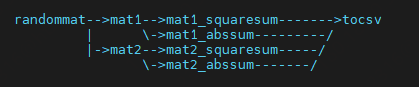
\includegraphics[height=50pt]{IMG/36.PNG}
\centering
\caption {computation graph}
\end{figure}

\FloatBarrier

In this example, \textbf{we only need to update the graph one time} to get following csv as output. In practice we can use a larger graph to generate different types of features for data mining purpose.

\begin{figure}[h]
\centering
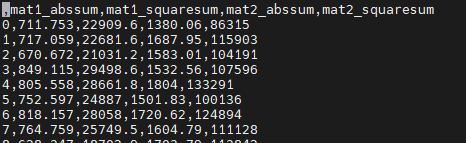
\includegraphics[height=60pt]{IMG/38.PNG}
\centering
\caption {output of main5}
\end{figure}

\FloatBarrier

\end{document}
